\begin{frame}{自己紹介(前回とほぼ変化なし)}
 \begin{tabular}[tb]{cc}

  \begin{minipage}{0.7\hsize}
   \begin{center}
    \begin{itemize}
     \item 榊原隆文 (twitter:@saka\_bar さかばー)
     \item すずかけ台の奥村研に所属
           \begin{itemize}
            \item 専門は自然言語処理
                  \begin{itemize}
                   \item テキスト集合からの知識獲得
                  \end{itemize}
           \end{itemize}
     \item 好きなもの
           \begin{itemize}
            \item 唐揚げ
            \item 凌駕
            \item Haskell
            \item IIDX DP
            \item 漢直(漢字直接入力)
                  \begin{itemize}
                   \item 紹介スライド
                  \end{itemize}
                  \href{http://www.slideshare.net/takafumisakakibara75/tutcode}{\structure{http://www.slideshare.net/takafumisakakibara75/tutcode}}
           \end{itemize}
    \end{itemize}
   \end{center}
  \end{minipage}

  \begin{minipage}{0.3\hsize}
   \begin{center}
    \begin{figure}[htbp]
     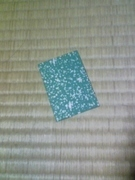
\includegraphics[bb=0 0 135 180,scale=0.5]{./figure/icon.jpg}
    \end{figure}
   \end{center}
  \end{minipage}

 \end{tabular}
\end{frame}

\begin{frame}{このスライドの特徴(前回とほぼ変化なし)}
 \begin{itemize}
  \item スライド作成のために\LaTeX のBeamerパッケージを利用
        \begin{itemize}
         \item PowerPointを使いたくない
         \item 前の発表の時にBeamerで痛い目見たけど、今回は大丈夫だろうか…
        \end{itemize}
  \item gitでバージョン管理
        % \begin{itemize}
  %  \item このスライドはタグのv0.1と対応
          % \end{itemize}
  \item ソースをgithubで公開
        \begin{itemize}
         \item \href{https://github.com/sakabar/prml_titech_8-1_8-2}{\structure{\url{https://github.com/sakabar/prml_titech_8-1_8-2}}}
        \end{itemize}
  \item PDFをSlideShareで公開
        \begin{itemize}
         \item \href{http://www.slideshare.net/takafumisakakibara75/slide-44207685}{\structure{\url{http://www.slideshare.net/takafumisakakibara75/slide-44207685}}}
        \end{itemize}
 \end{itemize}
\end{frame}
